\documentclass[bachelor,zhspacing]{cqu}  %单面打印版本
\usepackage{etex}
\def\tightlist{}

%%在这增加你需要的其它包
\definecolor{hellgelb}{rgb}{1,1,0.8}
\definecolor{colKeys}{rgb}{0,0,1}
\definecolor{colIdentifier}{rgb}{0,0,0}
\definecolor{colComments}{rgb}{1,0,0}
\definecolor{colString}{rgb}{0,0.5,0}
\usepackage{listings}
\lstset{%
    float=hbp,%
    basicstyle=\ttfamily\small, %
    identifierstyle=\color{colIdentifier}, %
    keywordstyle=\color{colKeys}, %
    stringstyle=\color{colString}, %
    commentstyle=\color{colComments}, %
    columns=flexible, %
    tabsize=4, %
    frame=single, %
    extendedchars=true, %
    showspaces=false, %
    showstringspaces=false, %
    numbers=left, %
    numberstyle=\tiny, %
    breaklines=true, %
   backgroundcolor=\color{hellgelb}, %
    breakautoindent=true, %
    captionpos=b,%
	xleftmargin=0pt%
}

\begin{document}

%-----------------------------------论文题目-------------------------------------------------
\xuehao{20121886}
\cntitle{基于卷积神经网络的人脸识别}
\cnauthor{李贝贝}
\cnmajor{软件工程}
\cnteacher{葛永新}
\cnxueyuan{软件学院}
\entitle{Face Recognization based on Convolutional Neural Network}
\enauthor{Beibei Li}
\enmajor{Software Engineering}
\enteacher{Prof. Yongxin Ge}
\enxueyuan{College of Software}
\cnkind{****}
\enkind{****}
%\cnzlteacher{ }  %%助理教师,如果必要,还要将cqu.cls中的有关该项前的%号去掉
%\enzlteacher{ }
\cndate{二O一六年六月}
\endate{June 2016}
%%%%只需修改上面的相关信息%%%%%%%%
\makecntitle 
\makeentitle 
%%%%%%%%%%%%%%%%%%%%%%%%%%%

\pagenumbering{Roman}
\setcounter{page}{0}
%------------------------------------文章摘要------------------------------------------------------------
\cnkeywords{卷积神经网络,人脸识别,深度学习 }
\begin{cnabstract}

卷积神经网络在提出时就凭借其出色的性能吸引了很多学者的兴趣,与深度学习理论结合,使之再次成为研究热点。
卷积神经网络引入了局部连接、权值共享和子采样的思想,与多层感知器相比大大降低了需要训练参数的数量。
而且在空间上其具有一定的平移、扭曲不变性。目前,卷积神经网络被广泛用到模式识别的各个领域。\par

人脸识别是模式识别领域一直以来的热点和重难点,采用卷积神经网络可以突破传统识别方法的瓶颈,具有重要的意义和价值。\par

本文旨在将卷积神经网络应用于人脸识别,围绕此目标,主要做了如下工作:

1.  总结和理解了感知器、多层感知器、梯度递减、后向传播等神经网络基础知识,学习卷积神经网络的主要思想和特点,理解其优越性
2.  将卷积神经网络用于人脸识别问题并将结果与其他识别方法对比分析。最终卷积神经网络以96.63\%的正确率超过其它方法,并远远超过传统方法。
3.  提取卷积神经网络的特征,与传统方法提取的特征比较分析。卷积神经网络的特征表现出更好的性能。

\end{cnabstract} 
\enkeywords{template, \LaTeX, abstract, paper}
\begin{enabstract}
     An abstract of a dissertation is a summary and extraction of 
research work and contributions. Included in an abstract should be 
description of research topic and research objective, brief 
introduction to methodology and research process, and summarization 
of conclusion and contributions of the research. An abstract should be 
characterized by independence and clarity and carry identical 
information with the dissertation. It should be such that the general 
idea and major contributions of the dissertation are conveyed
without reading the dissertation.\par
     An abstract should be concise and to the point. It is a 
misunderstanding to make an abstract an outline of the dissertation and 
words “the first chapter”, “the second chapter” and the like should be 
avoided in the abstract.\par
     Key words are terms used in a dissertation for indexing, 
reflecting core information of the dissertation. An abstract may 
contain a maximum of 5 key words, with semicolons used in between to 
separate one another.
\end{enabstract}
%%%%%%%%%%%%%%%%%%%%%%%%%%%%%%%%%%%%%%

%--------------文章目录-------------
\tableofcontents
\listoffigures
%\addcontentsline{toc}{section}{插图清单}
\listoftables
%\addcontentsline{toc}{section}{附表清单}


%------------------------------------词汇------------------------------------------------------------
\begin{denotation}{2.5}{0}

\item[cluster] 集群
\item[Itanium] 安腾
\item[SMP] 对称多处理
\item[API] 应用程序编程接口
\item[PI]   聚酰亚胺
\item[劝  学] 君子曰:学不可以已。青,取之于蓝,而青于蓝;冰,水为之,而寒于水。
  木直中绳。(车柔)以为轮,其曲中规。虽有槁暴,不复挺者,(车柔)使之然也。故木
  受绳则直, 金就砺则利,君子博学而日参省乎己,则知明而行无过矣。吾尝终日而思
  矣,  不如须臾之所学也;吾尝(足齐)而望矣,不如登高之博见也。登高而招,臂非加
  长也,  而见者远;  顺风而呼,  声非加疾也,而闻者彰。假舆马者,非利足也,而致
  千里;假舟楫者,非能水也,而绝江河,  君子生非异也,善假于物也。积土成山,风雨
  兴焉;积水成渊,蛟龙生焉;积善成德,而神明自得,圣心备焉。故不积跬步,无以至千
  里;不积小流,无以成江海。骐骥一跃,不能十步;驽马十驾,功在不舍。锲而舍之,朽
  木不折;  锲而不舍,金石可镂。蚓无爪牙之利,筋骨之强,上食埃土,下饮黄泉,用心
  一也。蟹六跪而二螯,非蛇鳝之穴无可寄托者,用心躁也。\pozhehao{} 荀况
\end{denotation}

%%%%%%%%%%%%%%%%%%%%%%%%%%%%%%%%%%%%%%%

\pagenumbering{arabic}

\section{绪论}\label{ux7eeaux8bba}

人脸识别是利用人脸识别算法对数字人脸信息进行身份识别的过程,完整的人脸识别流程为:从图片中检测人脸,然后对人脸进行识别,进而标识人脸身份。近几年来,卷积神经网络在模式识别领域取得了很好的效果,因此本文对卷积神经网络应用于人脸识别问题展开了研究和讨论。本章节主要包括人脸识别研究背景和意义,人脸识别系统的构成,人脸识别研究现状,深度学习研究现状等。

\subsection{人脸识别背景和意义}\label{ux4ebaux8138ux8bc6ux522bux80ccux666fux548cux610fux4e49}

随着互联网的迅猛发展,人们对信息安全的要求也越来越高。身份鉴定是保障信息安全的重要途径。每个人的生理特征具有唯一性、稳定性和客观性,通过识别生理特征可以唯一确定人的身份。近几年来,计算机视觉和人工智能发展迅猛,生物特征识别技术应运而生。通过传感器获取人的生理特征,再通过计算机、数学等知识进行分析,可以使计算机协助人们快速、便利地进行身份鉴定。

\begin{figure}[htbp]
\centering

\includegraphics{./pic/cqu.eps}
\caption{生物特征识别}\label{fig:}
\end{figure}

常见的生物特征识别技术有指纹识别、虹膜识别、人脸识别和行人再识别。其中人脸是身份信息最直观的表现方式,人脸识别技术是辨识自然人身份的重要手段,是其他计算机智能行为的基础。目前人脸识别已经应用于各行各业,并取得了很好的效果。在2008年中国举办奥运会期间,人脸识别技术便被用于奥运会的系统中,如今以人脸识别为基础的门禁系统更是随处可见。人脸识别的研究和应用给人们带来了极大的便利和安全保障。

一个完整的人脸识别系统应该包括人脸检测和人脸识别两个过程,如(\#fig:sys-fd-fr)

\begin{figure}[htbp]
\centering

\includegraphics{./pic/cqu.eps}
\caption{人脸检测与人脸识别}\label{fig:sys-fd-fr}
\end{figure}

人脸检测是指在图片中根据人脸结构特征,检测到人脸所在的区域并将人脸提取出来的过程。而人脸识别则是对比辨识以区分身份的过程,也是本文研究的重点,人脸识别的系统结构图如
图~\ref{fig:sys-constru}

\begin{figure}[htbp]
\centering

\includegraphics{./pic/cqu.eps}
\caption{人脸识别系统流程}\label{fig:sys-constru}
\end{figure}

人脸识别系统的完整流程是:首先通过人脸检测技术将人脸从背景图中分离出来,然后对人脸进行特征提取,再通过相似度度量区分身份。本文内容集中于人脸识别,对人脸身份进行判断。

\subsection{人脸识别研究现状}\label{ux4ebaux8138ux8bc6ux522bux7814ux7a76ux73b0ux72b6}

本文所讨论的人脸识别是通过对比人脸的特征值从而确定人脸身份的过程。人脸识别可以分为两个过程:特征提取和分类器选择。特征提取过程试图描述人脸信息的关键特征,而分类器的选择则直接影响了分类结果。目前用于人脸识别的方法主要有:几何结构发;基于子空间特征的方法,局部特征方法和深度学习方法。

几何结构法是通过利用一组几何特征矢量表示人脸面部拓扑结构的几何关系。该思想最初由Bledsoe与1966年提出,后IJ.Cox\textsuperscript{{[}1{]}},Huang\textsuperscript{{[}2{]}}等人改进。虽然基于几何结构的方法计算简单,但对特征点对齐要求非常高,从而大大限制了它的实用性。

基于子空间的方法的主要思想是将高维特征通过空间变换到一个低维的子空间中,使样本在低维空间中更容易分类。代表算法有:主成分分析PCA\textsuperscript{{[}3{]}}、线性判别分析LDA{[}{[}4{]};highleyman1962linear{]}、独立分量分析(Independent
Component Analysis,
ICA)\textsuperscript{{[}5{]}}。而后,在这三种算法上进行改进的算法不断涌现,例如与核技术相结合的KPCA\textsuperscript{{[}6{]}},核2DPCA\textsuperscript{{[}7{]}},核Fisherfaces\textsuperscript{{[}8{]}}。子空间的方法是在特征提取阶段所使用的方法,在保留人脸几何拓扑关系的同时也保留了部分局部特征。子空间是目前人脸识别最常用的特征方法,有计算量小,描述能力强,可分性好等优点。

局部特征方法主要思想是将人脸图像分解成多个局部特征,从而使特征分散,降低干扰因素的影响,局部特征方法较好地模拟了人类的识别能力,先对人脸的整体特征进行辨识,再对局部特征进行对比。代表方法有:由Ojala\textsuperscript{{[}9{]}}等提出的LBP特征、Lowe{[}{[}10{]};ke2004pca{]}提出的SIFT特征、由Daugman等提出的Gabor特征{[}{[}11{]};daugman1988complete{]}等。LBP特征的思想是讲一个局部的中心像素的灰度值设为阈值,将周围的像素点与阈值作比较转换成0和1,从而表示出局部的纹理。LBP特征具有旋转不变性和灰度不变性等优点。2010年,X.Tan和Triggs
Bill\textsuperscript{{[}12{]}}提出了局部三元模式(Local Ternary Pattern,
LTP)进一步扩展了LBP,使之描述能力更强。SIFT特征全名尺度不变特征变换(Scale
Invariant Feature Transform,
SIFT)特征,SIFT特征具有尺度不变性、位移不变性、仿射不变性和旋转不变性。SIFT通常和其他方法配合使用。Ke
Y\textsuperscript{{[}13{]}}于2004年提出PCA-SIFT方法;Gu
J\textsuperscript{{[}14{]}}于2009年提出了结合K-Means的聚类匹配算法。Gobar小波能够同时有效的描述人脸图像的局部特征和整体特征。

深度学习的主要思想是模仿人类的识别过程。由于在人脸识别过程中,样本数据会受到光照、姿势的影响。但人类在认知和识别过程中却几乎不会受这些因素的影响,这使人们考虑是否可以通过模拟人类而使计算机同样排除这样的干扰,准确地进行识别和判断。G.Hinton等\textsuperscript{{[}15{]}}等利用贪心注册那个算法训练DSNs,该模型可以在没有标签的情况下学习图像的低阶特征。Marc
Aurelio
Ranzato等\textsuperscript{{[}16{]}}将门控马尔科夫随机场(MRF)作为DBNs的前端从而学习人脸图像的深度生成模型。Osadchy
M
等\textsuperscript{{[}17{]}}利用卷积网络进行人脸检测,该模型是将原始图像映射到低维子空间中。Sun
Y\textsuperscript{{[}18{]}}等构建了基于三层卷积神经网络的级联回归结构。Huang
G B
等\textsuperscript{{[}19{]}}通过卷积深度信念网络(CDSN)来学习到了多层次的特征。Nair
和
Hinton\textsuperscript{{[}20{]}}使用深度学习进行目标识别和人脸验证,然而他们提出的模型由于不具有平移不变性,所以需要人工校正眼坐标。Sun
Y等\textsuperscript{{[}21{]}}提出受限玻尔兹曼机(RBM)和混合卷积神经网络(ConvNet)的网络模型,该算法在LFW数据库中表现出较好的性能。Lin
M
等\textsuperscript{{[}22{]}}提出使用深度信念网络解决姿态变化带来的非线性问题。Chen等\textsuperscript{{[}23{]}}将图像分割成不重叠的图像块,分别输入深度神经网络进行训练以解决图像过大的问题。Zhu
Z等\textsuperscript{{[}24{]}}提出FIP特征,以解决光照和姿态变化的问题。FIP特征显著减少类内差,比LBP,Gabor特征具有更好的鲁棒性。

与其他方法相比,利用神经网络和深度学习提取人脸特征,是对人脑工作原理的一种模拟,可以学习到更多人脸图像中的隐形特征,因此表现出很好的性能。

\subsection{卷积神经网络研究现状}\label{ux5377ux79efux795eux7ecfux7f51ux7edcux7814ux7a76ux73b0ux72b6}

二十世纪六十年代,Hubel和Wiesel\textsuperscript{{[}25{]}}在对猫的视觉皮层的研究中发现视网膜输出的信号在神经元传播的过程中经过了复杂的交换过程,而不是直接传入脑部的。视觉皮层中主要包括两类细胞:S(Simple)细胞和C(Complex)细胞。S细胞响应在自己感受野内的刺激
这个发现启发他们提出了感受域的概念。日本学者Fukushirna\textsuperscript{{[}26{]}}在八十年代基于感受域的概念提出了神经感知机,视觉层中的S细胞和C细胞分别对应S神经元和C神经元。S神经元负责特征抽取,C神经元主要负责以C神经元的输出作为输入并以更大的感受野感受刺激。此外,他还发现了在神经网络中对于小区域上的一组参数,在整个物体中具有位移不变性,并且在物体发生扭曲或者其他形变时仍然能够很好地识别。Trotin\textsuperscript{{[}27{]}}等人提出了动态调节神经感知机的神经元个数的方案,称之为动态蛇精感知机。主要思想是学习时将神经元初始化为零,然后在学习过程中根据实际情况逐渐假如神经元,直到找到合适的神经网络。学习过程中,根据反馈信号自动调整,节省了大量人工参与的精力。而后,很多研究人员对卷积神经网络提出了改进方案,Alexander和Taylor\textsuperscript{{[}28{]}}等人将各种优化方式结合起来,提出了``改进感知机''理论。

目前,卷积神经网络的应用非常广泛,而在最初的手写体字符识别问题上,更是取得了99.77\%的卓越效果,远远超过其他模式识别的方式。卷积神经网络的优点是原始图像不需做特殊的处理,因此节省了大量图片预处理的工作。LeCun\textsuperscript{{[}29{]}},Mathew
Browne\textsuperscript{{[}30{]}},satoshi
Yamaguchi\textsuperscript{{[}31{]}}在图像处理领域使用了卷积神经网络,并取得了很好的效果。之后,卷积神经网络被陆续用在了语音识别\textsuperscript{{[}32{]}},人脸识别\textsuperscript{{[}33{]}},行人检测\textsuperscript{{[}34{]}},机器人导航\textsuperscript{{[}35{]}},人体动作识别\textsuperscript{{[}36{]}}等多个领域。

\subsection{论文组织结构}\label{ux8bbaux6587ux7ec4ux7ec7ux7ed3ux6784}

人脸识别在现代社会中具有愈加重要的作用,高准确率和高效率是人脸识别追求的目标。深度学习凭借其对人脑工作原理的模拟,在模式识别中表现出良好的性能。本文将卷积神经网络运用于人脸识别并进行探索和研究。主要研究工作包括:

\begin{enumerate}
\def\labelenumi{\arabic{enumi}.}
\tightlist
\item
  通过阅读卷积神经网络的相关文献,仔细学习了感知器、多层感知器、后向传播算法等背景知识,理解了卷积神经网络的特征、结构以及应用方向等。学习了softmax分类器和支持向量机分类器等常用分类器的原理。
\item
  将卷积神经网络应用于人脸识别,并通过对隐藏节点个数,过滤器个数等参数微调使之效果更好。
\item
  将通过卷积神经网络提取的特征值,分别输入softmax分类器和支持向量机分类器中,对比结果并分析
\item
  分别通过卷积神经网络提取的特征值与其他方法所提取的特征值输入至支持向量机,对比结果并分析。
\end{enumerate}

本文中各章的内容组织结构如下:

第一章主要介绍人脸识别的研究意义、背景和现状以及人脸识别系统的结果,卷积神经网络的研究现状等。
第二章介绍了卷积神经网络的相关知识:感知器、多层感知器、梯度下降法和后向传播学习。
第三章描述了卷积神经网络的主要思想、网络拓扑结构和常用分类器等内容。
第四章将卷积神经网络运用于人脸识别,并在实验结果上和其他方法进行了对比和分析。
第五章提出了卷积神经网络与支持向量机相结合的人脸识别框架,将卷积神经网络提取的特征输入至支持向量机进行分类,并对实验结果分析。

\section{相关知识}\label{ux76f8ux5173ux77e5ux8bc6}

\subsection{感知器}\label{ux611fux77e5ux5668}

\subsubsection{概念}\label{ux6982ux5ff5}

感知器的思想于1957年由Frank
Rosenblatt被提出。在机器学习中,感知器是用于处理监督学习下的二元分类问题。它的输入值是样本的特征向量\(x\),输出值为二值函数\(f(x)\),称为感知器的激活函数如:

\begin{displaymath}
y = \left\{ \begin{array}{ll}
 1 & \textrm{if $\omega \cdot x + b > 0$}\\
 0 & \textrm{otherwise}
  \end{array} \right.
\end{displaymath}

其中,\(\omega\)是输入向量\(x\)中各值对应权值所构成的向量,\(\omega \cdot x\)是求两者的内积,即\(\sum_{i = 0}^{m}\omega_{i}x_{i}\),其中\(m\)是输入向量所包含数值的个数。\(b\)是偏移项,其值不取决于输入的任何一项,是可训练的。

\subsubsection{构造方法}\label{ux6784ux9020ux65b9ux6cd5}

为了构造一个感知器,我们需要定义一些变量:

\begin{itemize}
\tightlist
\item
  \(y = f(z)\):输入向量\(z\)到输出值的映射函数。
\item
  \(D = {(x_{1},x_{1},\ldots,(x_{s},d_{s}))}\):包含\(s\)个样本的训练集:
  其中:

  \begin{itemize}
  \tightlist
  \item
    \(x_{j}\)是n维输入向量,\(x_{j,i}\)表示第\(j\)个输入向量中的第\(i\)个特征值,\(x_{j,0}=1\)
  \item
    \(d_{j}\)是输入向量对应的输出值
  \end{itemize}
\item
  \(\alpha\):模型的学习率。其中\(0<\alpha\le 1\)
\end{itemize}

关于感知器结构中的权重,我们利用\(\omega_{i}\)来表示权重向量中的第\(i\)个值,将会与输入向量中的第\(i\)个特征值相乘;在前面我们定义\(x_{j,0} = 1\),因此\(w_{0}\)对应的就是我们定义的偏移量\(b\)。利用\(\omega_{i}(t)\)表示第\(t\)次学习的权重

感知器的结构可表示为如图 图~\ref{fig:slp_construct}

\begin{figure}[htbp]
\centering

\includegraphics{./pic/cqu.eps}
\caption{单层感知器结构图}\label{fig:slpux5fconstruct}
\end{figure}

\subsubsection{学习算法}\label{ux5b66ux4e60ux7b97ux6cd5}

感知器的学习目的是寻找一个超平面能够使正负样本实例完全正确分开。样本的实际输出值与期望输出值的平均残差函数为:

\[\frac{1}{s}\sum_{j = 1}^{s}\lvert d_{j}-y_{j}(t)\rvert\]

感知器的优化目标应该使残差最小,理想的情况为0,但在实际应用中,往往有一定的容错率。可以定义容错阈值\(\gamma\),当目标函数小于\(\gamma\)时,则停止学习。

学习过程如下:

\begin{enumerate}
\def\labelenumi{\arabic{enumi}.}
\tightlist
\item
  初始化权重\(\omega\)和阈值\(\gamma\)。权重可以被初始化为0或者其他的小随机数。
\item
  对于训练集\(D\)中的每个样本\(j\),我们对输入值\(x_{j}\)与期望输出\(d_{j}\)执行以下步骤:

  \begin{itemize}
  \tightlist
  \item
    计算实际输出:\(y_{j}(t)= f[w(t)\cdot x_{j}]\)
  \item
    更新权值:对于所有\(0\le i \le n\),计算\(\omega_{i}(t+1) = \omega_{i}(t) + \alpha(d_{j} - y_{j}(t))x_{j,i}\)
  \end{itemize}
\item
  训练至残差小于设定的阈值即可停止训练。
\end{enumerate}

感知器是一个线性分类器,Frank
Rosenblatt证明了如果一个两类模式是线性可分的,则一定存在一个超平面可以将它们分开。

\subsection{多层感知器}\label{ux591aux5c42ux611fux77e5ux5668}

感知器可以很好地解决两类线性分类问题,然而却无法解决非线性问题,例如
图~\ref{fig:xor} XOR问题:

\begin{figure}[htbp]
\centering
\includegraphics{./pic/xor.eps}
\caption{异或问题示意图}\label{fig:xor}
\end{figure}

单个感知器虽然无法解决异或问题,但多个感知器组合则可以实现复杂空间的分割。如
图~\ref{fig:mlp-xor}

\begin{figure}[htbp]
\centering

\includegraphics{./pic/cqu.eps}
\caption{多感知器解决异或问题}\label{fig:mlp-xor}
\end{figure}

单个感知器可以将空间一分为二,在第一个感知器的基础上第二个感知器即可实现异或,因此多个感知器配合可以解决非线性分类问题。

\subsubsection{网络结构}\label{ux7f51ux7edcux7ed3ux6784}

感知器是多层感知器的基本组成。多层感知器模拟人类神经的工作原理,将每一个感知器模拟人类神经的神经元的基础功能:来自外界的电信号通过突触传递给神经元,当细胞收到的信号综合超过一定阈值后,细胞被激活,通过轴突向下一个细胞发送电信号,完成对外界信息的加工。

多层感知器除输入和输出层以外,还包括至少一层以上的隐藏层,且层与层之间是全连接,即多层感知器与上一层的每一个感知器都有连接。多层感知器的结构图如
图~\ref{fig:mlp-con}

\begin{figure}[htbp]
\centering

\includegraphics{./pic/cqu.eps}
\caption{多感知器结构图}\label{fig:mlp-con}
\end{figure}

\subsubsection{激活函数}\label{ux6fc0ux6d3bux51fdux6570}

感知器中的函数\(f\)称为激活函数,若激活函数为线性函数,则利用线性代数的知识,网络输出的任意层都可以被转换成标准的输入-输出两层模型。因此在多层感知器中,激活函数采用非线性函数以达到非线性分类的目的。

常用的激活函数为\(y(v_{i}) = tanh(v_{i})\)和\(y(v_{i}) = (1+e^{-v_{i}})^{-1}\)。前者是值域处于(-1,1)之间的双曲正切函数,后者是logistic函数,值域在(0,1)。前者是有后者变换而得到,两者形状很相似,两者的图像如
图~\ref{fig:mlp-act}

\begin{figure}[htbp]
\centering
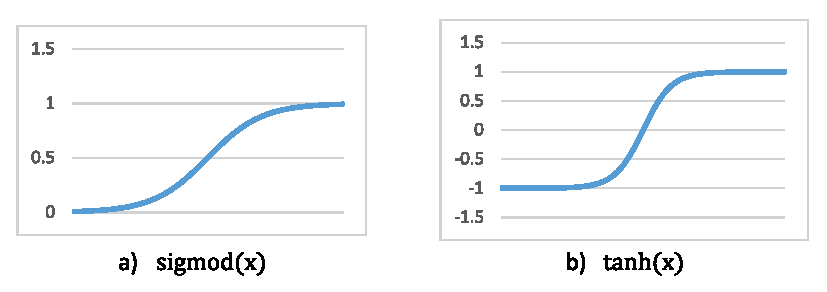
\includegraphics{./pic/tanh-sigmod.eps}
\caption{激活函数图像}\label{fig:mlp-act}
\end{figure}

\subsubsection{梯度下降法}\label{ux68afux5ea6ux4e0bux964dux6cd5}

梯度下降法是一种最优化算法,可以用来优化神经网络结构的参数,由于其原理是寻找最快下降的方向进行优化,因此也称为最快下降法。

梯度是标量场中某一点上指向标量场增长最快的方向,是一个向量场,梯度的长度即为该点最大的变化率。对于一个单变量的实值函数,梯度就是倒数。对于二元函数\(f(x,y)\),若函数\(f(x,y)\)在平面区域\(D\)中具有一阶偏导数,则对于点\(f(x,y)\in D\),梯度为\(gradf(x,y) = \frac{\partial f}{\partial x}\vec{i} + \frac{\partial f}{\partial y}\vec{j}\),类似的对于三元函数\(f(x,y,z)\),梯度为\(\frac{\partial f }{\partial x }\vec{i} + \frac{\partial f }{\partial y }\vec{j} + \frac{\partial f }{\partial z }\vec{k}\),其中\(\vec{i},\vec{j},\vec{k}\)分别为x,y,z轴方向的单位向量。因此一个标量函数的梯度可以记为:\(\nabla{\phi}\)或者\(grad\phi\),其中\(\nabla\)表示微分算子。

若实值函数\(F(x)\)在点\(a\)处可微且有定义,则函数\(F(x)\)在\(a\)点沿着梯度相反的方向\(-\nabla{\phi}\)下降最快。因而,如果\(b = a - \gamma \nabla F(a)\)成立,其中
\(\gamma > 0\)为一个足够小的数值,那么\(F(a)\ge F(b)\)。因此从初始值\(x_{0}\)出发,考虑如下序列\(x_{0},x_{1},x_{2},\ldots\)使得
\[x_{n+1} = x_{n} - \gamma_{n}\nabla F(x_{n}),n\ge 0\] 因此可以得到
\[F(x_{0})\ge F(x_{1})\ge F(x_{2})\ge\ldots,\]
最终使\((x_{n})\)收敛到期望的极值,如 图~\ref{fig:mlp-grad-1}。

\begin{figure}[htbp]
\centering

\includegraphics{./pic/cqu.eps}
\caption{梯度下降法极值收敛过程}\label{fig:mlp-grad-1}
\end{figure}

梯度下降法的局限性在于由于初值设定随机,可能会陷入局部最小,而不是全局最小,如
图~\ref{fig:mlp-grad-2}

\begin{figure}[htbp]
\centering

\includegraphics{./pic/cqu.eps}
\caption{梯度下降法收敛至局部最优}\label{fig:mlp-grad-2}
\end{figure}

\subsubsection{后向传播学习}\label{ux540eux5411ux4f20ux64adux5b66ux4e60}

感知器的学习目标是使实际输出结果和期望输出结果之间的误差最小,通过后向传播实现。后向传播包括两个过程:传播和权重更新

\begin{itemize}
\tightlist
\item
  传播

  \begin{itemize}
  \tightlist
  \item
    向前传播:将数据输入至神经网络中,得到输出结果
  \item
    向后传播:利用实际输出与期望输出的误差计算对所有神经元的梯度
  \end{itemize}
\item
  更新权重

  \begin{itemize}
  \tightlist
  \item
    利用学习率计算权重更新的变化量
  \item
    将变化量更新至权重
  \end{itemize}
\end{itemize}

后向传播的算法流程如 图~\ref{fig:mlp-bp}

\begin{figure}[htbp]
\centering

\includegraphics{./pic/cqu.eps}
\caption{后向传播的算法流程}\label{fig:mlp-bp}
\end{figure}

以常见的平方误差为例,误差函数为: \[ E = \frac{1}{2}(t-y)^{2}\]
其中\(E\)表示平方误差,\(t\)是训练数据的期望输出,\(y\)是实际输出,\(\frac{1}{2}\)是为了后续计算微分是时方便而加上的系数,不会影响最终优化结果。有感知器的计算原理可知,对于神经元\(j\),它的输出\(o_{j}\)应为:
\[o_{j}=\phi(net_{j}) = \phi(\sum_{k = 1}^{n}\omega_{kj}o_{k})\]
激活函数的输入\(net_{j}\)等于网络上一层中各个感知器输出的加权之和,当计算输入数据后的第一层网络输出结果时,则是将输入数据进行加权求和。激活函数\(\phi\)是非线性且可微的,以logistic函数为例:
\[\phi(z) = \frac{1}{1+e^{-z}}\] 求导得:
\[\frac{d_{\phi}}{d_{z}}(z) = \phi(z)(1-\phi(z))\]
根据梯度下降法原理,我们采用链式求导求解误差对权值的偏微分:
\begin{equation}\frac{\partial E}{\partial w_{ij}} = \frac{\partial E}{\partial o_{j}}\frac{\partial o_{j}}{\partial net_{j}}\frac{\partial net_{j}}{\partial \omega_{ij}}\label{eq:bp-d}\end{equation}
其中:
\begin{equation}\frac{\partial net_{j}}{\partial \omega_{ij}} = \frac{\partial}{\partial \omega_{ij}}(\sum_{k = 1}^{n}\omega_{kj}o_{k})=o_{j}\label{eq:bp-d-1}\end{equation}

\begin{equation}\frac{\partial o_{j}}{\partial net_{j}} = \frac{\partial}{\partial net_{j}}\phi(net_{j}) = \phi(net_{j})(1-\phi(net_{j}))\label{eq:bp-d-2}\end{equation}
对于输出层神经元,即\(o_{j} = y\):

\begin{equation}\frac{\partial E}{\partial o_{j}} = \frac{\partial E}{\partial y} = \frac{\partial}{\partial y}\frac{1}{2}(t-y)^2 = y-t\label{eq:bp-d-3-1}\end{equation}

对于非输出层神经元,我们可以将\(E(o_{j})\)是所有将神经元\(j\)的输出作为输入的神经元\(L = u,v,\ldots,w\)的误差函数:
\begin{equation}\frac{\partial E}{\partial o_{j}} = \sum_{l\in L}(\frac{\partial E}{\partial net_{l}}\frac{\partial net_{l}}{\partial o_{j}} = \sum_{l\in L}(\frac{\partial E}{\partial o_{l}}\frac{\partial o_{l}}{\partial net_{l}}\omega_{jl}))\label{eq:bp-d-3-2}\end{equation}
将
公式~\ref{eq:bp-d},公式~\ref{eq:bp-d-1}, \ref{eq:bp-d-2}, \ref{eq:bp-d-3-1}, \ref{eq:bp-d-3-2}组合,得到:

\[\frac{\partial E}{\partial \omega_{ij}}= \delta_{j} o_{i}\] 其中:
\begin{equation}
\delta_{j} =\frac{\partial E}{\partial o_{j}} \frac{\partial o_{j}}{\partial net_{j}} = \left\{ \begin{array}{ll}
 (o_{j}-t_{j})o_{j}(1-o_{j})) & \textrm{$j$ 为输出层神经元,}\\
 (\Sigma_{l\in L}\delta_{l}\omega_{jl})o_{j}(1-o_{j}) & \textrm{ $j$ 为非输出层神经元}
  \end{array} \right.
\label{eq:bp-d-delta}\end{equation}

此时,可以对权重进行更新了,为了使目标值向降低的方向优化,我们需要乘上-1,权重更新的步长由学习率\(\alpha\)确定:

\begin{equation}
\Delta\omega_{ij} = -\alpha\frac{\partial E}{\partial \omega_{ij}}= \left\{ \begin{array}{ll}
 -\alpha o_{j}(o_{j}-t_{j})o_{j}(1-o_{j})) & \textrm{$j$ 为输出层神经元,}\\
 -\alpha o_{j}(\Sigma_{l\in L}\delta_{l}\omega_{jl})o_{j}(1-o_{j}) & \textrm{ $j$ 为非输出层神经元}
  \end{array} \right.
\label{eq:bp-d-delta-weight}\end{equation}

\section{卷积神经网络}\label{ux5377ux79efux795eux7ecfux7f51ux7edc}

\subsection{概述}\label{ux6982ux8ff0}

卷积神经网络(Convolutional Neural
Networks)是多层感知器的变体,是目前模式识别的研究热点。它的提出源于对猫的视觉皮层细胞的研究,1962年Hubel和Wiesel提出了感受野(receptive
field)的概念,1984年此概念在日本学者Fukushima提出的神经认知机(neocognitron)中首次被应用。神经认知机将一个视觉模式分解成许多子模式(特征)然后进入分层递阶式相连的特征平面进行处理,尝试在物体有位移或轻微变形的时候,也能完成识别。神经认知机可以看做第一个卷积神经网络的实现。

卷积神经网络的主要特点体现在两个方面:局部连接,权值共享和子采样。局部连接是指层与层神经元之间的连接采用局部连接代替全连接;权值共享是指同一层中神经元之间的连接权值是共享的;子采样是对得到的特征图进行特征采样。三者使卷积神经网络在很大程度上降低了参数数量,从而使网络的复杂度降低。由于其结构与生物神经网络非常相似,即使输入的图像不做任何预处理,卷积神经网络的识别效果也比较显著,同时避免了繁琐的特征提取的过程。
本章将详细介绍卷积神经网络的基本思想、拓扑结构和常用分类器。

\subsection{主要思想}\label{ux4e3bux8981ux601dux60f3}

根据Hubel和Wiesel对猫初级视皮层的研究,生物的初级视皮层包括简单细胞和复杂细胞,简单细胞主要负责感知其感受野内的特定边缘刺激,而复杂细胞则以简单细胞的输出为输入,并负责以更大的感受野来感受边缘刺激。根据简单细胞和复杂细胞的工作原理,卷积神经网络主要采用三种结构来进行视皮层的模拟:局部连接、权值共享以及子采样。

\subsubsection{局部连接}\label{ux5c40ux90e8ux8fdeux63a5}

局部连接是指在相邻层之间不使用全连接而使用局部连接,从而不仅减少了需要训练的参数数量,而且利用了图像的局部特征信息。

如 图~\ref{fig:cnn-locallink-1}
所示,图a为全连接,图b为局部连接。假设图片有\(1000\times1000\)个像素的图片,有一百万的隐层神经元,全连接需要每一个隐层神经元连接到图像的每一个像素点,有\(100\times 100\times 1000000 = 10^{12}\)个连接,也就需要\(10^{12}\)个参数。局部连接则只需要每个节点只与其感受野中的像素点进行相连,假设其感受野为\(10\times 10\),则一百万个隐层神经元就只要\(10\times 10\times 100000 = 10^{8}\)个权值参数,权值参数的个数减少四个数量级。因此局部连接减少了所需训练的权值参数。

\begin{figure}[htbp]
\centering

\includegraphics{./pic/cqu.eps}
\caption{全连接与局部连接}\label{fig:cnn-locallink-1}
\end{figure}

如
图~\ref{fig:cnn-locallink-2所示},每一层神经元只与其前一层的神经元存在局部连接,第I层的神经元连接了I-1层神经元的3个相邻的神经元,第I+1层与第I层的连接也有类似的规则,I+1层的神经元虽然相对于第I层的接受域宽度为3,但其相对于第I-1层的接受域却为5,这种结构经过多个层堆叠在一起之后,会使得过滤器逐渐成为全局,但却包含了低层的很多局部信息,因此局部连接可以利用图像的局部信息。通常在实际应用中,利用多个局部连接的过滤器可以利用图像的多种局部特征。

\begin{figure}[htbp]
\centering

\includegraphics{./pic/cqu.eps}
\caption{局部连接结构图}\label{fig:cnn-locallink-2}
\end{figure}

\subsubsection{权值共享}\label{ux6743ux503cux5171ux4eab}

在上节例子中通过局部连接,所需训练参数有了数量级上的减少,但仍然需要训练\(10^{8}\)个参数,这意味着如果想要得到有意义的参数,则需要样本容量大于\(10^{8}\),而如此庞大的样本容量常常不易达到,即便可以达到,网络的结构也会异常复杂,训练结果精确度也不会很高,而权值共享则可以很好地解决这个问题。

权值共享是指在相邻层神经元连接时都采用相同的权值,如
图~\ref{fig:cnn-sharedweight-1所示},不同的线条形状代表不同的权值,相同的线条形状代表相同权值,则上节例子中,若局部连接的感受野为10*10,则只需要100个权值,因此大大降低了所需权值数量。此外,由于权值共享使权值以同样的方向和距离出现,因此权值共享使卷积神经网络具有平移不变性。

\begin{figure}[htbp]
\centering

\includegraphics{./pic/cqu.eps}
\caption{权值共享示意图}\label{fig:cnn-sharedweight-1}
\end{figure}

通过局部连接和权值共享,并以卷积的方式在输入的每个位置提取输入的局部特征,卷积神经网络有效模拟了视皮层中的简单细胞。

\subsubsection{子采样}\label{ux5b50ux91c7ux6837}

子采样操作是对得到的特征图进行特征映射(特征采样),在水平和竖直的方向利用\(w\times w\)的连续子区域以\(s\)为步长进行特征映射,其中\(1\le s\le w\),当\(s = w\)时,采样子区域之间没有重叠部分,否则,采样区域间有重叠部分。常用的映射方法是最大值映射和平均值映射,即在\(w\times w\)的子区域中,选取最大值或者计算子区域中的平均值作为该区域的映射值。如@fig:cnn-sample-1所示,特征图的大小为\(4\times 4\),若采用\(2\times 2\)的连续子区域以2为步长进行子采样,采样后的特征图为\((4/2)\times (4/2)\),即\(3 \times 3\)。可以看出子采样减少了神经元的数目,相同的神经元个数代表了更大的感受野,很好地模拟了视皮层复杂细胞。

\begin{figure}[htbp]
\centering

\includegraphics{./pic/cqu.eps}
\caption{子采样示意图}\label{fig:cnn-sample-1}
\end{figure}

\subsection{网络拓扑结构}\label{ux7f51ux7edcux62d3ux6251ux7ed3ux6784}

卷积神经网络的传统模型是由多层特征提取阶段与一个分类器组成的结构,输入的特征在经过多层的特征映射学习到高层特征之后,利用在最后一个阶段得到的特征被输入分类器进行分类。通常在应用中,卷积神经网络一共有1-3个特征映射阶段,每个特征映射阶段包括卷积层和子采样层。
LeNet-5是一个用于手写体识别的网络结构,本节将以此为例展开介绍,LeNet-5结构如
图~\ref{fig:cnn-topol-lenet}。

\begin{figure}[htbp]
\centering

\includegraphics{./pic/cqu.eps}
\caption{LeNet-5结构图}\label{fig:cnn-topol-lenet}
\end{figure}

\subsubsection{卷积层}\label{ux5377ux79efux5c42}

卷积层是卷积神经网络的重要组成部分。卷积层将前一层的一个或者多个特征图与一个或者多个卷积核进行卷积操作,输出特征图中的相邻神经元共享大部分的输入特征图中的神经元。对于一个大小\(m\times n\)的特征图,用大小\(k\times k\)的卷积核进行卷积操作,输出特征图的大小为\((m-k=1)\times (k-k+1)\)。如
\textbf{???}
所示,一个大小为\(5\times 5\)的卷积核在图像大小为\(8\times 8\)上进行卷积,得到的输出特征图像为\(4 \times 4\)

\begin{figure}[htbp]
\centering

\includegraphics{./pic/cqu.eps}
\caption{卷积层示意图}\label{fig:cnn-topol-c}
\end{figure}

一般在卷积操作之后,会在结果上加一个偏置参数,此偏置参数是可训练的。此外,为了使神经网络具有非线性的拟合性能,需要一个非线性的激活函数,通过该函数映射后最终得到卷基层的输出特征图。

以LeNet-5结构为例,第一层、第三层和第五层为卷积层,在其第一个卷积层中,输入图像为原始图像,大小为\(28\times 28\),8个大小为\(5 \times 5\)的卷积核卷积后得到8张大小为\(28\times 28\)的特征图。在第三层中同样采用\(5 \times 5\)的卷积核卷积得到20张大小为\(10\times 10\)的特征图,第五层为一个全连接层,产生一个与原始输入图像对应的特征向量,也是要输入到分类器进行分类的向量。

\subsubsection{子采样层}\label{ux5b50ux91c7ux6837ux5c42}

子采样层对卷积层的输出特征图进行采样,采样区域的宽度和高度可以根据实际情况进行调节。在采样子区域没有重叠的情况下,一张大小为\(m\times n\)的输入特征图,经过\(w\times h\)的尺度进行采样,则得到的图像大小应为\((m/w)\times (n/h)\)

在LeNet-5中第二层和第四层为子采样层,在第二层中,通过\(2\times 2\)的尺度进行子采样,将大小为\(28\times 28\)的图像采样为\(14\times14\)的图像,同理在第四层中,将大小为\(10\times 10\)的输入图像采样为\(5\times 5\)的输出图像。

\subsubsection{分类器}\label{ux5206ux7c7bux5668}

分类器是将得到最终输出的特征向量进行分类的分类器。常用的分类器有logistic回归模型以及其扩展softmax分类或者一层或两层的神经网络。在LeNet-5中用的是softmax
分类器。

以上就是基本的卷积神经网络结构,在实际应用中,卷积和子采样的层数、卷积过滤器的维数、子采样采样子区域的维数等参数都是可调节的。可以根据具体情况提出有效的网络结构。

\subsection{常用分类器}\label{ux5e38ux7528ux5206ux7c7bux5668}

卷积神经网络一般利用softmax回归模型、支持向量机或者一个两到三层的神经网络作为分类器,本文主要涉及softmax回归模型和支持向量机。

\subsubsection{softmax分类器}\label{softmaxux5206ux7c7bux5668}

softmax分类器是用softmax回归模型进行分类。softmax回归模型是logistic模型在多类分类问题上的推广,能够有效解决多类问题,例如手写题识别问题需要分十类,此时logistics无法达到目的,但softmax却可以很好地解决。

在理解softmax分类器之前,需要先了解logistic模型。在logistic模型中,训练集由\(m\)个有标记的样本组成:\({(x^{(1)},y^{(1)}),\ldots,(x^{(m)},y_{(m)})}\),输入特征\(x^{(i)} \in R^{n+1}\),与感知器理论中相似,特征向量\(x\)的维度为\(n+1\)项,其中\(x_{0} = 1\)
对应偏移量。类标记\(y_{(i)}\in{0,1}\)。logistic的假设函数为:

\[h_{\theta}(x)=\frac{1}{1+\exp(-\theta^{T}x)}\] 代价函数如下:
\begin{equation}J(\theta) = - \frac{1}{m}[\sum_{i=1}^{m}y^{(i)}\log h_{\theta}+(1+y^{(i)})log(1-h_{\theta}(x^{(i)})))]\label{eq:logistic-cost}\end{equation}
训练logistic的过程是通过训练参数\(\theta\)从而使代价函数的值最小。

在softmax回归中,样本的标记可以取\(k\)个值,\(y^{(i)}\in {1,2,\ldots,k}\)。注意此处的下标是从1开始。

对于softmax的假设函数,我们希望能够分别估算出某一样本分别属于各类的概率值\(p(y=j|x)\)。因此假设函数需要输出一个表示属于\(k\)类的概率值估计的\(k\)维向量,所以,softmax的假设函数\(h_{\theta}(x)\)形式如下:

\[
    h_{\theta}(x^{(i)})=
        \left[
            \begin{array}{ccc}
                p(y^{(i)}=1|x^{(i)};\theta)\\
                p(y^{(i)}=2|x^{(i)};\theta)\\
                \vdots\\
                p(y^{(i)}=k|x^{(i)};\theta)
            \end{array}
        \right]=
        \frac{1}{\Sigma_{j = 1}^{k}e^{\theta_{j}^{T}x^{(i)}}}
        \left[
            \begin{array}{ccc}
                e^{\theta_{1}^{T}x^{(i)}}\\
                e^{\theta_{2}^{T}x^{(i)}}\\
                \vdots\\
                e^{\theta_{k}^{T}x^{(i)}}
            \end{array}
        \right]
\]
其中,\(\theta_{1},\theta_{2},\ldots,\theta_{k}\)为模型参数,\(\frac{1}{\Sigma_{j=1}^{k}e^{\theta_{j}^{T}x^{(i)}}}\)是对概率进行归一化,使所有概率之和为1。

我们定义\(1\{\cdot\}\)为示性函数,\(1\{\textrm{值为真的表达式}\}=1\);\(1\{\textrm{值为假的表达式}\}=0\)
logistic代价函数如 公式~\ref{eq:logistic-cost} 所示,同时可以改写成:
\[J(\theta) = -\frac{1}{m}[\sum_{i=1}^{m}\sum_{j=0}^{1}1\{y^{(i)\}=j}\log p(y^{(i)} = j|x^{(i)};\theta)]\]
在softmax函数中将样本\(x\)分为类别\(j\)的概率为:
\[p(y^{(i)}=j|x^{(i)};\theta)=\frac{e^{\theta_{j}^{T}x^{(i)}}}{\Sigma_{l=1}^{k}e^{\theta_{j}^{T}x^{(i)}}}\]
softmax的代价函数表达式为:
\[J(\theta)= -\frac{1}{m}[\sum_{i=1}^{m}\sum_{j=1}^{k}1{y^{(i)}=j}\log \frac{e^{\theta_{j}^{T}x^{(i)}}}{\Sigma_{l=1}^{k}}e^{\theta_{l}^{T}x^{(i)}}]\]
softmax代价函数的梯度为:
\[\nabla_{\theta_{j}}J(\theta) = -\frac{1}{m}\sum_{i=1}^{m}[x^{(i)}(1\{y^{(i)}=j\}-p(y^{(i)}=j|x^{(i)};\theta))]\]
其中\(\nabla_{\theta_{j}}J(\theta)\)的第\(l\)个元素\(\frac{\partial J(\theta)}{\partial\theta_{jl}}\)是\(J(\theta)\)对\(\theta_{j}\)的第\(l\)个分量的偏导数。
将其代入梯度下降法中,每一次迭代更新如下:
\[\theta_{j}:=\theta_{j}-\alpha\nabla_{\theta_{j}}J(\theta)(j=1,\ldots,k)\]

\subsubsection{支持向量机}\label{ux652fux6301ux5411ux91cfux673a}

支持向量机以统计学习理论为基础,可以很好地处理回归问题、分类问题和判别分析等诸多问题。并在预测和综合评价等问题中也表现出很好的效果。本文主要将支持向量机用于分类问题。

\paragraph{线性支持向量机}\label{ux7ebfux6027ux652fux6301ux5411ux91cfux673a}

支持向量机的原理在于寻找一个最优分类超平面能够在满足分类要求的同时最大化超平面两侧的空白区域。如@fig:svm-linear

\begin{figure}[htbp]
\centering

\includegraphics{./pic/cqu.eps}
\caption{线性SVM原理示意图}\label{fig:svm-linear}
\end{figure}

已两类线性分类为例,给定训练数据集\((x_{i},y_{i}),i=1,2,ldots,l,x\in R^{n},y\in{1,-1}\),将超平面记做\((\omega\cdot x_{i})+b=0\),其中\(\omega\)是一个\(n\)维向量,b是一个常量。为使分类将所有样本分类正确并有分类间隔,需要满足约束:\(y_{i}[w\cdot x_{i}+b]\ge\quad\quad i = 1,2,\ldots,n\)

可以计算出分类间隔为\(2/\lvert \omega \rvert\),因此求解最优化超平面可以转化成如下约束式进行求解:
\[\min\Phi(\omega) = \frac{1}{2}\lvert \omega \rvert^{2} = \frac{1}{2}(\omega^{,}\cdot\omega)\]
为了解决这个问题,引入拉格朗日函数:
\(L(\omega,b,a)=\frac{1}{2}\lvert\omega\rvert-a(y((\omega\cdot x) + b)-1)\)
其中,\(a_{i}>0\)为拉格朗日乘数。最优解由拉格朗日函数的鞍点决定,最优化解应在鞍点处\(\omega\)和\(b\)
的偏导为0,将该问题转换成相应的对偶问题即: \[maxQ(a) = 
\begin{array}{lll}
\sum_{j=1}^{l}a_{j}-\frac{1}{2}\sum_{i=1}^{l}\sum_{j=1}^{l}a_{i}a_{j}y_{i}y_{j}(a_{i}\cdot x_{j}) & \\
s.t.\quad \sum_{j=1}^{l}a_{j}y_{j}=0 & j=1,2,\ldots,l,a_{j}\ge0,j=1,2,\ldots,l
\end{array}\] 计算最优解为\(a^{*}=(a_{1}^{})\)
最优权值向量和最优偏移量,分别为:

\[\omega^{*} = \sum_{j=1}^{l}a_{j}^{\*}y_{j}x_{j}\]
\[b^{*} = y_{i}-\sum_{j=1}^{l}y_{j}a_{j}^{\*}(x_{j}\cdot x_{i})\]

其中,下标\(j\in{j|a_{j}^{*}>0}\)。得到最优分类超平面\((\omega^{\*}\cdot x) + b^{\*}\),最优分类函数为:

\[
\begin{array}{ll}
f(x)=sgn\{(\omega^{*}\cdot x)+b^{\*}\}=\\
sgn\{(\sum_{j=1}^{l}a_{j}^{*}y_{j}(x_{j}\cdot x_{i}))+b^{\*}\},x\in R^{n}
\end{array}
\]

\paragraph{非线性支持向量机}\label{ux975eux7ebfux6027ux652fux6301ux5411ux91cfux673a}

对于非线性问题,支持向量机的主要思想是先将输入数据映射到一个高维空间中,使数据在高维空间中线性可分。设从\(x\)做从输入空间到\(R^{n}\)到高维特征空间\(H\)的变换为\(\Phi\),得:
\[x\to\Phi(x)=(\Phi_{1}(x),\Phi_{2}(x),\ldots,\Phi_{l}(x))^{T}\]
以特征向量\(\Phi(x)\)代替输入向量\(x\),可以得到非线性最有分类函数为:
\begin{equation}
\begin{array}{ll}
f(x)=sgn\{(\omega^{*}\cdot \Phi(x))+b^{\*}\}=\\
sgn\{(\sum_{j=1}^{l}a_{j}^{*}y_{j}(\Phi(x_{j})\cdot \Phi(x_{i}))+b^{\*}\},x\in R^{n}
\end{array}
\label{eq:svm-nolear}\end{equation}
而寻找合适的映射函数\(\Phi\)是非常复杂,不容易实现。仔细观察@eq:svm-nolear,可以发现最优分类超平面只与内积\(<x_{i},x_{j}>\)有关,因此支持向量机引入核函数来完成从线性到非线性的变换。常用的核函数有:

\begin{enumerate}
\def\labelenumi{\arabic{enumi}.}
\tightlist
\item
  多项式核函数:\(K(x_{i},K_{j})=(x_{1}^{T}x_{1})^{d}\)
\item
  Gauss径向基核函数:\(K(x_{i},K_{j})=\exp(-q\lvert x_{1}-x_{2}\rvert^{2})\)
\item
  其他一些核函数有B-样条函数,Fourier核函数,双曲正切函数等。
\end{enumerate}

\paragraph{多类分类问题}\label{ux591aux7c7bux5206ux7c7bux95eeux9898}

支持向量机本来是针对二类分类问题的,但在现实中,却又很多问题是多类分类问题,如手写体识别问题等。对于多类分类问题,支持向量集主要有两种解决方案:

\begin{enumerate}
\def\labelenumi{\arabic{enumi}.}
\tightlist
\item
  将K类分类问题分解成K个二类分类问题。对每个分类器按照是否属于该类别分为正负样本,在经过K个分类器之后,K个类别的数据都被分离开来。
\item
  通过一对一的方法,每次将种类二分,并将样本分为两类,然后再对分得的子集分成两类,继续分类,如此递归,共需要构造\(C_{k}^{2}\)个分类。
\end{enumerate}

\section{基于卷积神经网络的人脸识别}\label{ux57faux4e8eux5377ux79efux795eux7ecfux7f51ux7edcux7684ux4ebaux8138ux8bc6ux522b}

本章节将卷积神经网络的理论用于人脸识别,给出实验结果,并对实验结果与其他人脸识别方法进行对比分析。

\subsection{YaleB数据集}\label{yalebux6570ux636eux96c6}

Yale人脸库是美国耶鲁大学创建的人脸数据库,共包含15人,每人11张照片,在表情和光照条件下有所变化。YaleB人脸数据集\textsuperscript{{[}37{]}}则是Yale数据库的扩展,扩展的部分包含16128幅图像,28个人,每人包括9种姿态,64种光照条件,图片为PGM格式,图片为\(168\times 192\)。耶鲁大学还提供了扩展Yale数据库的裁剪版,将人脸范围裁剪下来,形成\(32\times 32\),共39(28+11)个人,除去由于拍摄等原因损坏的照片,总共2414张图片,每人有效图片数量大约在60-64张之间。图~\ref{fig:yaleb}
是YaleB人脸库原图和裁剪图的部分样本

\begin{figure}[htbp]
\centering

\includegraphics{./pic/cqu.eps}
\caption{YaleB人脸库}\label{fig:yaleb}
\end{figure}

在本文的实验中,我们在每种人脸数据图像中随机抽取5张,共190张作为测试集,同理抽样190张作为验证集。其余图像全部作为网络的训练集,由于样本数量的限制,实验中将测试集同时当作验证集来使用。

\subsection{网络设计}\label{ux7f51ux7edcux8bbeux8ba1}

这里采用与Le-Net5相似的结构,如图~\ref{fig:cnn-net}。参数设置情况如
表~\ref{tbl:cnn-params}

\begin{figure}[htbp]
\centering

\includegraphics{./pic/cqu.eps}
\caption{网络设计图}\label{fig:cnn-net}
\end{figure}

\begin{longtable}[]{@{}lr@{}}
\caption{\label{tbl:cnn-params}卷积神经网络参数表 }\tabularnewline
\toprule
参数名称 & 参数值\tabularnewline
\midrule
\endfirsthead
\toprule
参数名称 & 参数值\tabularnewline
\midrule
\endhead
卷积层过滤器大小 & \(5\times 5\)\tabularnewline
卷积层过滤器个数 & 10,20\tabularnewline
子采样层过滤器大小 & \(2\times 2\)\tabularnewline
隐藏全连接层节点个数 & 2000\tabularnewline
学习率 & 0.05\tabularnewline
权值向量\(\omega\)初值 & \(\vec{0}\)\tabularnewline
偏移量\(b\)初值 & 0\tabularnewline
\bottomrule
\end{longtable}

\subsection{网络实现}\label{ux7f51ux7edcux5b9eux73b0}

\subsubsection{网络训练与测试流程}\label{ux7f51ux7edcux8badux7ec3ux4e0eux6d4bux8bd5ux6d41ux7a0b}

在实验中,设置迭代次数(epoch)为400次,即所有数据将会被输入模型训练400次,每组(patch)输入数据包括40张人脸数据。实验设置停止条件为:当连续超过1000个实例的训练数据都没有使验证集的误判率降低,训练停止。从而使在模型能够找到最优解的同时,防止过拟合。每输入100次数据则会将验证集输入模型进行验证。网络运行流程图如
\textbf{???}

\begin{figure}[htbp]
\centering

\includegraphics{./pic/cqu.eps}
\caption{网络训练与测试流程图}\label{fig:cnn-flow}
\end{figure}

\subsubsection{编码实现}\label{ux7f16ux7801ux5b9eux73b0}

Theano是一个引入了多维矩阵计算的基于Python的库,它支持大规模的科学计算;与Python的基础科学计算包NumPy紧紧结合;并且可以使用GPU,在浮点数的计算上速度超过CPU高达140倍;此外,它有动态的C语言生成器,使数学计算更快。Theano中提供了一些深度学习所用的基本函数,例如:卷积函数\(conv()\),下采样函数\(downsample()\)等。文档给出了简单的卷积神经网络的Demo,方便了我们构建卷积神经网络。下面给出关键代码

\begin{itemize}
\tightlist
\item
  卷积层与下采样层
\end{itemize}

\begin{verbatim}
class ConvPoolLayer(object):
    def __init__(self, rng, input, filter_shape, image_shape,
     poolsize=(2, 2)):
        assert image_shape[1] == filter_shape[1]
        self.input = input
        fan_in = numpy.prod(filter_shape[1:])
        fan_out = (filter_shape[0] * 
                    numpy.prod(filter_shape[2:]) /
                    numpy.prod(poolsize))
        # 初始化
        W_bound = numpy.sqrt(6. / (fan_in + fan_out))
        self.W = theano.shared(
            numpy.asarray(
                rng.uniform(low=-W_bound, high=W_bound, 
                            size=filter_shape),
                dtype=theano.config.floatX
            ),
            borrow=True
        )
        b_values = numpy.zeros((filter_shape[0],), 
                   dtype=theano.config.floatX)
        self.b = theano.shared(value=b_values, borrow=True)
        # 卷积
        conv_out = conv.conv2d(
            input=input,
            filters=self.W,
            filter_shape=filter_shape,
            image_shape=image_shape
        )
        # 子采样
        pooled_out = downsample.max_pool_2d(
            input=conv_out,
            ds=poolsize,
            ignore_border=True
        )
        self.output = T.tanh(pooled_out + 
                        self.b.dimshuffle('x', 0, 'x', 'x'))
        # 保存参数
        self.params = [self.W, self.b]
\end{verbatim}

\begin{itemize}
\item
  隐藏全连接层

\begin{verbatim}
class HiddenLayer(object):
def __init__(self, rng, input, n_in, n_out, W=None,
             b=None,activation=T.tanh):
    self.input = input
    if W is None:
        W_values = numpy.asarray(
            rng.uniform(
                low=-numpy.sqrt(6. / (n_in + n_out)),
                high=numpy.sqrt(6. / (n_in + n_out)),
                size=(n_in, n_out)
            ),
            dtype=theano.config.floatX
        )
        if activation == theano.tensor.nnet.sigmoid:
            W_values *= 4
        W = theano.shared(value=W_values, name='W', 
                        borrow=True)
    if b is None:
        b_values = numpy.zeros((n_out,), 
                            dtype=theano.config.floatX)
        b = theano.shared(value=b_values, name='b',
                            borrow=True)
    self.W = W
    self.b = b
    lin_output = T.dot(input, self.W) + self.b
    self.output = (
        lin_output if activation is None
        else activation(lin_output)
    )
    # parameters of the model
    self.params = [self.W, self.b]
\end{verbatim}
\item
  softmax分类器
\end{itemize}

\begin{verbatim}
class LogisticRegression(object):
    def __init__(self, input, n_in, n_out):
        self.W = theano.shared(
            value=numpy.zeros(
                (n_in, n_out),
                dtype=theano.config.floatX
            ),
            name='W',
            borrow=True
        )
        self.b = theano.shared(
            value=numpy.zeros(
                (n_out,),
                dtype=theano.config.floatX
            ),
            name='b',
            borrow=True
        )
        self.p_y_given_x = T.nnet.softmax(
                            T.dot(input, self.W) + self.b)
        self.y_pred = T.argmax(self.p_y_given_x, axis=1)
        self.params = [self.W, self.b]

    def negative_log_likelihood(self, y):
        return -T.mean(T.log(self.p_y_given_x)
                        [T.arange(y.shape[0]), y])

    def errors(self, y):
        if y.ndim != self.y_pred.ndim:
            raise TypeError(
              'y should have the same shape as self.y_pred',
                ('y', y.type, 'y_pred', self.y_pred.type)
            )
        if y.dtype.startswith('int'):
            return T.mean(T.neq(self.y_pred, y))
        else:
            raise NotImplementedError()
\end{verbatim}

\begin{itemize}
\tightlist
\item
  网络结构构造
\end{itemize}

\begin{verbatim}
    layer0_input = x.reshape((batch_size, 1, 32, 32))
    # 第一层卷积+子采样
    layer0 = LeNetConvPoolLayer(
        rng,
        input=layer0_input,
        image_shape=(batch_size, 1, 32, 32),
        filter_shape=(nkerns[0], 1, 5, 5),
        poolsize=(2, 2)
    )
    # 第二层卷积+子采样,输入为上一层的输出:
    # 上一层卷积后得到:(32-5+1 ,32-5+1) = (28, 28)
    # 上一层后得到: (28/2, 28/2) = (14, 14)
    layer1 = LeNetConvPoolLayer(
        rng,
        input=layer0.output,
        image_shape=(batch_size, nkerns[0], 14, 14),
        filter_shape=(nkerns[1], nkerns[0], 5, 5),
        poolsize=(2, 2)
    )
    # 全连接层
    layer2_input = layer1.output.flatten(2)
    layer2 = HiddenLayer(
        rng,
        input=layer2_input,
        n_in=nkerns[1] * 5 * 5,
        n_out=2000,
        activation=T.tanh
    )
    #分类器
    layer3 = LogisticRegression(input=layer2.output, 
                        n_in=2000, n_out=38)   
    # 代价函数
    cost = layer3.negative_log_likelihood(y)
\end{verbatim}

\subsection{对比实验}\label{ux5bf9ux6bd4ux5b9eux9a8c}

\subsubsection{PCA-KNN}\label{pca-knn}

PCA,Principal Component
Analysis,主成分分析。是基础的数学分析方法,其实际应用十分广泛,是一种常用的多变量分析方法。其主要思想,是探索如何利用少数的主要成分来代表数据中的大部分信息。主成分分析在大大降低维度的同时,能够保持原始数据中大部分信息不被丢失,因此常常被用作数据降维。

KNN,K Nearest
Neighbor,K-最近邻方法。是一种有监督的分类算法,也是最简单的机器学习方法之一。其理论已经比较成熟。主要思想是对于一个新的输入实例,在训练集中找与之最邻近的K个实例,若K个实例中大多数属于某个类,就将此输入分入到该类中。KNN算法思想简单易懂,得到了广泛的应用。

文献 {[}38{]}
中,在YaleB数据集上利用PCA对图像数据进行处理,利用少数的维度代表原始数据的信息,完成提取特征的过程,然后利用KNN做分类器做出了实验。

\subsubsection{LPP-KNN}\label{lpp-knn}

LPP\textsuperscript{{[}39{]}},Locality Preserving
Projection,局部保持投影,是一种无监督的学习算法。是流形学习方法Laplacian
Eigenmap的线性表示,既能避免了PCA\textsuperscript{{[}40{]}}等传统线性方法不能表示原始数据中非线性流形的缺陷\textsuperscript{{[}41{]}},又能解决非线性方法不易得到新样本点低维投影的问题\textsuperscript{{[}42{]}}。该算法的主要思想在于通过保持高维数据内在的局部流形结构,来构造出拉普拉斯矩阵来指导降维,从而得到显式的投影矩阵。该算法在人脸识别等问题中能够成功应用。

文献 {[}38{]}
中,在YaleB数据集上利用LPP提取特征,KNN做分类器做出了实验。

\subsubsection{LBP-DBN}\label{lbp-dbn}

LBP全称Local Binary
Pattern、局部二值模式,是一个经典的纹理特征描述子,于1994年有Ojala\textsuperscript{{[}9{]}}提出,经过多次改进\textsuperscript{{[}43,44{]}},现在的LBP算子具备了一定的光照不变性和旋转不变性,能够描述角、点、边缘等图像中的细节。一般为了提高旋转不变性和光照不变性,通常会将分块和LBP描述子结合起来,从而提取的纹理特征,既有局部特征又有全局特征。

DBN全称Deep Belief
Network、深度信念网络,是一种由受限玻尔兹曼机构成的一种人工神经网络,通过贪心学习算法来进行学习。也经常被用于特征识别、分类问题等领域。

文献 {[}45{]}
中采用分块与LBP结合的方法提取特征并使用深度信念网络进行分类,并在Yale扩展数据库YaleB上进行了实验。

\subsection{实验结果与分析}\label{ux5b9eux9a8cux7ed3ux679cux4e0eux5206ux6790}

经过实验,卷积神经网络在YaleB数据库上达到了96.63\%的正确率,训练过程中误判率的变化图像如
图~\ref{fig:cnn-err}
。通过图像可知,卷积神经网络最初的错误率达到99\%到100\%,这主要是由于网络权值和偏移量参数的初值设为零导致。但通过训练,很快错误率急速下降至10\%以内,而后收敛速度慢慢降下来,但仍在不断地收敛,最后错误率到达3.375\%时网络结束训练。卷积神经网络在人脸识别的过程中错误率由最初几乎100\%下降到3.375\%,足以说明其超强的自学习能力。

\begin{figure}[htbp]
\centering
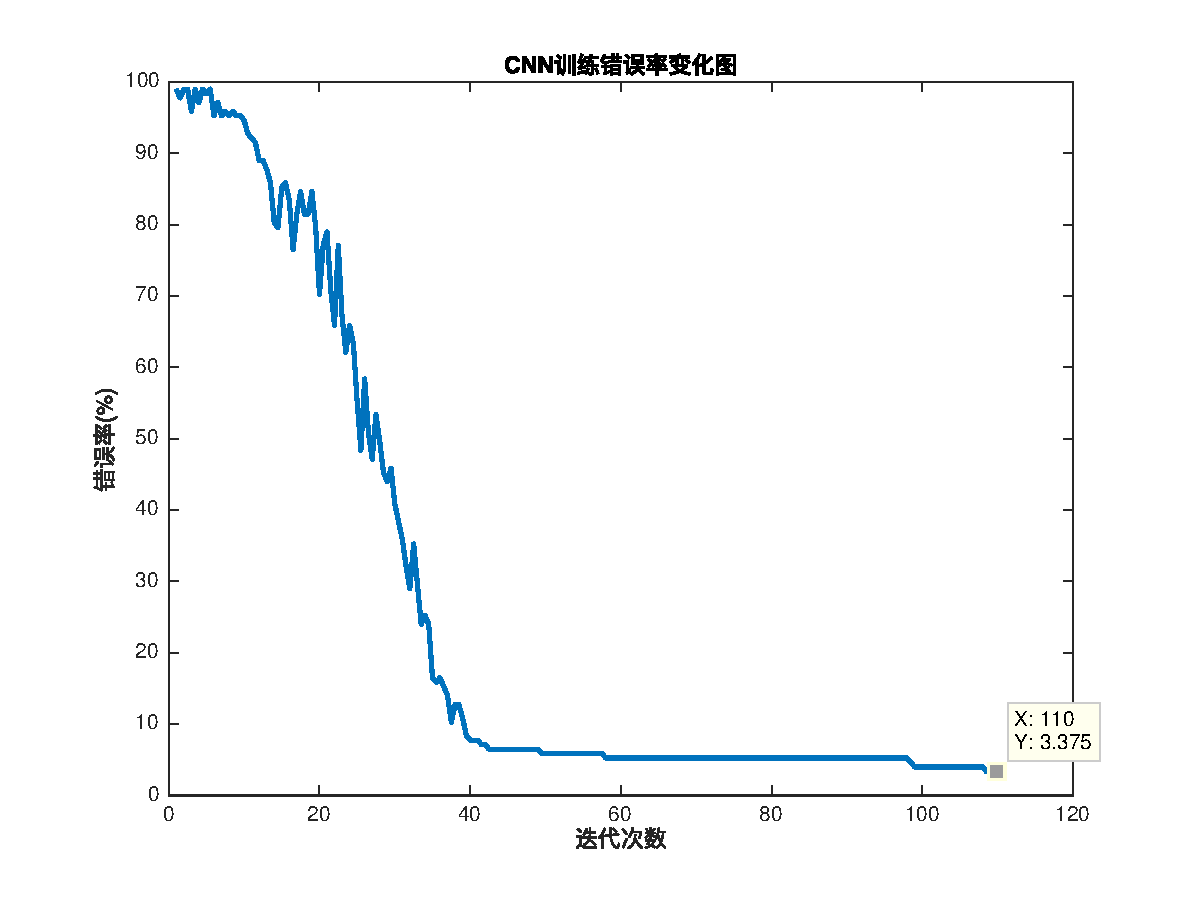
\includegraphics[width=5.72917in]{./pic/cnn-err.eps}
\caption{CNN误判率变化图}\label{fig:cnn-err}
\end{figure}

再将卷积神经网络与其他的人脸识别方法作比较,主成分分析和K最近邻算法相结合能够使正确率稳定在74.75\%左右,局部保持投影和K最近邻结合效果比起主成分分析,在87.05\%左右,卷积神经网络的识别结果。此外我们可以发现LBP特征和深度信念网络结合的识别方法效果虽也不如卷积神经网络得到的结果,但比起前两种要接近得多。深度信念网络也是一种深度学习的方法,进一步验证了深度学习方法的有效性。

\begin{longtable}[]{@{}ll@{}}
\caption{\label{tbl:cnn-res}多种方法下人脸识别正确率对比
}\tabularnewline
\toprule
方法 & 最佳识别率\tabularnewline
\midrule
\endfirsthead
\toprule
方法 & 最佳识别率\tabularnewline
\midrule
\endhead
PCA+KNN\textsuperscript{{[}38{]}} & 74.75\%\tabularnewline
NPE+KNN\textsuperscript{{[}38{]}} & 87.05\%\tabularnewline
LBP+DBN\textsuperscript{{[}45{]}} & 96.17\%\tabularnewline
CNN & 96.63\%\tabularnewline
\bottomrule
\end{longtable}

\section{基于卷积神经网络的人脸特征研究}\label{ux57faux4e8eux5377ux79efux795eux7ecfux7f51ux7edcux7684ux4ebaux8138ux7279ux5f81ux7814ux7a76}

本章对卷积神经网络所提取的特征进行探究。卷积神经网络在分类问题上的突出表现,与它对特征的学习是密切相关的。卷积和采样使之能够很好地捕捉到图片信息的细节,多层过滤器更是加强了其描述特征的能力。因此对卷积神经网络所提取的特征的探究是非常有意义的。在本章中,将卷积神经网络与局部二值特征(LBP)\textsuperscript{{[}9,43,44{]}}和方向梯度特征(HOG)两种经典的特征提取方式作比较。

\subsection{实验设计}\label{ux5b9eux9a8cux8bbeux8ba1}

本实验为对比实验,分别提取卷积神经网络训练得到的特征、局部二值特征和梯度方向特征。分类器统一使用支持向量机。最后将三种特征得到的分类结果进行对比,分析卷积神经网络的优劣势。注意,在支持向量机分类过程中,YaleB训练集属于分类问题,需要将数据分为39类。

\subsubsection{实验一:基于卷积神经网络的人脸特征}\label{ux5b9eux9a8cux4e00ux57faux4e8eux5377ux79efux795eux7ecfux7f51ux7edcux7684ux4ebaux8138ux7279ux5f81}

在第四章的实验中,我们已经实现了使用卷积神经网络(CNN)实现了人脸识别。为了提取卷积神经网络训练得到的数据,

\begin{enumerate}
\def\labelenumi{\arabic{enumi}.}
\tightlist
\item
  训练卷积神经网络至误判率不再优化,停止训练。
\item
  保存误判率达到最小时网络的参数。
\item
  利用参数重构网络至全连接层。
\item
  将原始训练集和测试集数据输入网络得到全连接层的数据即是通过该卷积神经网络训练得到的数据结果。
\end{enumerate}

分别将训练集和测试集输入至支持向量机中进行训练和测试。

\subsubsection{实验二:局部二值特征}\label{ux5b9eux9a8cux4e8cux5c40ux90e8ux4e8cux503cux7279ux5f81}

局部二值特征(LBP,Local Binary
Pattern)\textsuperscript{{[}9,43,44{]}}是非常常用的人脸识别特征。用来描述图像局部纹理特征,其主要思想是通过将周围像素与中心像素的灰度值进行比较,用0和1对整幅图像重新编码,得到的仍然是一张图像。为了解决由于``位置没有对准''而造成的较大误差,加入直方图的思想。所以LBP特征的提取过程为:

\begin{enumerate}
\def\labelenumi{\arabic{enumi}.}
\tightlist
\item
  将图片转成灰度图像。
\item
  将检测图像分成小区域,如\(16\times 16\)。
\item
  对于小区域中的每个像素,将与之相邻的8个灰度与其进行比较,如果周围像素值大于中心像素值,则将该像素置1,否则将该像素置0。
\item
  计算每个小区域内的直方图,并进行归一化操作。
\item
  将每个小区域连接的统计直方图连接成为一个特征向量,就形成了整个图像的LBP纹理特征向量。
\end{enumerate}

同理我们将训练集和测试集进行提取LBP特征的操作,将结果输入SVM进行训练和测试。

\subsubsection{实验三:方向梯度直方图}\label{ux5b9eux9a8cux4e09ux65b9ux5411ux68afux5ea6ux76f4ux65b9ux56fe}

方向梯度直方图(HOG,Histogram of Oriented
Gradient)特征\textsuperscript{{[}46{]}}是一种用于物体检测的特征描述子,在文献
{[}46{]}
即是法国学者Dalal提出利用HOG和SVM进行行人检测。HOG特征的主要思想任务局部目标的表象和特征可以通过梯度或者边缘的方向密度函数表示出来。提取HOG特征的过程如下:

\begin{enumerate}
\def\labelenumi{\arabic{enumi}.}
\tightlist
\item
  灰度化:将图片转成灰度图片,图片信息变成\((x,y,z)\)三维数据,\((x,y)\)表示在图片上的像素点坐标,z表示该坐标像素下的灰度值。
\item
  颜色空间归一化:一般采用Gamma矫正法,目的在于调节图像的对比度,降低光照变化带来的影响。
\item
  计算梯度:计算图像中每个像素的梯度,捕捉轮廓信息。
\item
  统计梯度直方图:划分细胞单元,并统计单元细胞中的梯度直方图。
\item
  计算块内梯度直方图:将细胞单元合并成面积更大的块,并在块内将梯度直方图归一化。
\end{enumerate}

收集HOG特征:将所有块中的直方图向量收集起来组合成一个大的HOG特征向量,即为该图像的特征向量。

提取HOG特征后,输入SVM进行训练和测试。

\subsection{实验实现}\label{ux5b9eux9a8cux5b9eux73b0}

此实验的实现主要使用MATLAB和Python实现。其中,局部二值特征和方向梯度直方图的提取和收集采用MATLAB实现,其他部分采用Python实现,并且使用了sklearn库。sklearn是一个Python的科学计算库,提供了包括分类、聚类、回归、降维等多种模式识别的方法,包括支持向量机,利用sklearn库可以方便地实现支持向量机的各种情况,包括多类问题等。

\subsection{实验结果与分析}\label{ux5b9eux9a8cux7ed3ux679cux4e0eux5206ux6790-1}

三种特征提取方法对人脸提取的特征如 图~\ref{fig:egi-face}

\begin{figure}[htbp]
\centering

\includegraphics{./pic/cqu.eps}
\caption{三种方法特征脸对比}\label{fig:egi-face}
\end{figure}

三种特征的分类结果如 表~\ref{tbl:res-fea} :

\begin{longtable}[]{@{}lccc@{}}
\caption{\label{tbl:res-fea}多种特征识别正确率 }\tabularnewline
\toprule
方法 & 卷积神经网络 & 局部二值特征 & 方向梯度直方图\tabularnewline
\midrule
\endfirsthead
\toprule
方法 & 卷积神经网络 & 局部二值特征 & 方向梯度直方图\tabularnewline
\midrule
\endhead
正确率 & 0 & 0 & 0\tabularnewline
\bottomrule
\end{longtable}

\section{总结和展望}\label{ux603bux7ed3ux548cux5c55ux671b}

\subsection{全文总结}\label{ux5168ux6587ux603bux7ed3}

卷积神经网络在提出时就引起了广大科研学者们的兴趣。深度学习以来,又掀起了对其研究的高潮。其在各领域的应用效果也比较明显。本文章结合人脸识别问题,主要做了以下工作:

\begin{enumerate}
\def\labelenumi{\arabic{enumi}.}
\tightlist
\item
  了解了人脸识别相关技术、卷积神经网络的发展和现状;深度理解了感知器、多层感知器的工作方式,以及卷积神经网络的主要思想和特点;同时也了解了深度学习的相关方法,对模式识别、计算机视觉有了全新的认识。
\item
  将卷积神经网络应用于人脸识别问题,并将结果与其他人脸识别技术相比较,更加验证了卷积神经网络和深度学习在模式识别中的杰出效果。
\item
  将卷积神经网络训练到的特征与其他特征方法做比较,并通过实验说明其优越性。
\end{enumerate}

\subsection{未来展望}\label{ux672aux6765ux5c55ux671b}

在日常生活中,收集无标签的人脸数据集要比收集有标签的数据集容易的多,其他领域也是这样,例如在行人再识别问题中,大量的视频监控会产生海量的无标签行人数据,因此,在卷积神经网络的基础上发展无监督学习算法将会很有帮助。此外,大量的训练数据,多层的网络结构,以及每层中大量的网络节点,都使深度神经网络的计算变得日益复杂,研究提高计算效率的有效方式也将会给深度学习的发展带来极大的便利。

\hypertarget{refs}{}
\hypertarget{ref-cox1996feature}{}
{[}1{]} COX I J, GHOSN J, YIANILOS P N. Feature-based face recognition
using mixture-distance{[}C{]}//Computer Vision and Pattern Recognition,
1996. Proceedings CVPR'96, 1996 IEEE Computer Society Conference on.
IEEE, 1996: 209--216.

\hypertarget{ref-huang1992human}{}
{[}2{]} HUANG C-L, CHEN C-W. Human facial feature extraction for face
interpretation and recognition{[}J{]}. Pattern recognition, Elsevier,
1992, 25(12): 1435--1444.

\hypertarget{ref-jolliffe2002principal}{}
{[}3{]} JOLLIFFE I. Principal component analysis{[}M{]}. Wiley Online
Library, 2002.

\hypertarget{ref-fisher1936use}{}
{[}4{]} FISHER R A. The use of multiple measurements in taxonomic
problems{[}J{]}. Annals of eugenics, Wiley Online Library, 1936, 7(2):
179--188.

\hypertarget{ref-jutten1991blind}{}
{[}5{]} JUTTEN C, HERAULT J. Blind separation of sources, part I: An
adaptive algorithm based on neuromimetic architecture{[}J{]}. Signal
processing, Elsevier, 1991, 24(1): 1--10.

\hypertarget{ref-scholkopf1997kernel}{}
{[}6{]} SCHÖLKOPF B, SMOLA A, MÜLLER K-R. Kernel principal component
analysis{[}G{]}//Artificial Neural Networks---ICANN'97. Springer, 1997:
583--588.

\hypertarget{ref-sun2008efficient}{}
{[}7{]} SUN N, WANG H-x, JI Z-h, 等. An efficient algorithm for Kernel
two-dimensional principal component analysis{[}J{]}. Neural Computing
and Applications, Springer, 2008, 17(1): 59--64.

\hypertarget{ref-liu2004improving}{}
{[}8{]} LIU Q, LU H, MA S. Improving kernel Fisher discriminant analysis
for face recognition{[}J{]}. Circuits and Systems for Video Technology,
IEEE Transactions on, IEEE, 2004, 14(1): 42--49.

\hypertarget{ref-ojala1996comparative}{}
{[}9{]} OJALA T, PIETIKÄINEN M, HARWOOD D. A comparative study of
texture measures with classification based on featured
distributions{[}J{]}. Pattern recognition, Elsevier, 1996, 29(1):
51--59.

\hypertarget{ref-brown2002invariant}{}
{[}10{]} BROWN M, LOWE D G. Invariant Features from Interest Point
Groups.{[}C{]}//BMVC. 2002.

\hypertarget{ref-daugman1985uncertainty}{}
{[}11{]} DAUGMAN J G. Uncertainty relation for resolution in space,
spatial frequency, and orientation optimized by two-dimensional visual
cortical filters{[}J{]}. JOSA A, Optical Society of America, 1985, 2(7):
1160--1169.

\hypertarget{ref-tan2010enhanced}{}
{[}12{]} TAN X, TRIGGS B. Enhanced local texture feature sets for face
recognition under difficult lighting conditions{[}J{]}. Image
Processing, IEEE Transactions on, IEEE, 2010, 19(6): 1635--1650.

\hypertarget{ref-ke2004pca}{}
{[}13{]} KE Y, SUKTHANKAR R. PCA-SIFT: A more distinctive representation
for local image descriptors{[}C{]}//Computer Vision and Pattern
Recognition, 2004. CVPR 2004. Proceedings of the 2004 IEEE Computer
Society Conference on. IEEE, 2004, 2: II--506.

\hypertarget{ref-gu2009enhancement}{}
{[}14{]} GU J, ZHOU J, CHEN X. An enhancement of k-means clustering
algorithm{[}C{]}//Business Intelligence and Financial Engineering, 2009.
BIFE'09. International Conference on. IEEE, 2009: 237--240.

\hypertarget{ref-hinton2006fast}{}
{[}15{]} HINTON G E, OSINDERO S, TEH Y-W. A fast learning algorithm for
deep belief nets{[}J{]}. Neural computation, MIT Press, 2006, 18(7):
1527--1554.

\hypertarget{ref-ranzato2011deep}{}
{[}16{]} RANZATO M A, SUSSKIND J, MNIH V, 等. On deep generative models
with applications to recognition{[}C{]}//Computer Vision and Pattern
Recognition (CVPR), 2011 IEEE Conference on. IEEE, 2011: 2857--2864.

\hypertarget{ref-osadchy2007synergistic}{}
{[}17{]} OSADCHY M, CUN Y L, MILLER M L. Synergistic face detection and
pose estimation with energy-based models{[}J{]}. The Journal of Machine
Learning Research, JMLR. org, 2007, 8: 1197--1215.

\hypertarget{ref-sun2013deep}{}
{[}18{]} SUN Y, WANG X, TANG X. Deep convolutional network cascade for
facial point detection{[}C{]}//Proceedings of the IEEE Conference on
Computer Vision and Pattern Recognition. 2013: 3476--3483.

\hypertarget{ref-le2011learning}{}
{[}19{]} LE Q V, ZOU W Y, YEUNG S Y, 等. Learning hierarchical invariant
spatio-temporal features for action recognition with independent
subspace analysis{[}C{]}//Computer Vision and Pattern Recognition
(CVPR), 2011 IEEE Conference on. IEEE, 2011: 3361--3368.

\hypertarget{ref-nair2010rectified}{}
{[}20{]} NAIR V, HINTON G E. Rectified linear units improve restricted
boltzmann machines{[}C{]}//Proceedings of the 27th International
Conference on Machine Learning (ICML-10). 2010: 807--814.

\hypertarget{ref-sun2013hybrid}{}
{[}21{]} SUN Y, WANG X, TANG X. Hybrid deep learning for face
verification{[}C{]}//Proceedings of the IEEE International Conference on
Computer Vision. 2013: 1489--1496.

\hypertarget{ref-li2010low}{}
{[}22{]} LI B, CHANG H, SHAN S, 等. Low-resolution face recognition via
coupled locality preserving mappings{[}J{]}. Signal Processing Letters,
IEEE, IEEE, 2010, 17(1): 20--23.

\hypertarget{ref-chen2013modular}{}
{[}23{]} CHEN X, XIAO B, WANG C, 等. Modular hierarchical feature
learning with deep neural networks for face verification{[}C{]}//Image
Processing (ICIP), 2013 20th IEEE International Conference on. IEEE,
2013: 3690--3694.

\hypertarget{ref-zhu2013deep}{}
{[}24{]} ZHU Z, LUO P, WANG X, 等. Deep learning identity-preserving
face space{[}C{]}//Proceedings of the IEEE International Conference on
Computer Vision. 2013: 113--120.

\hypertarget{ref-hubel1962receptive}{}
{[}25{]} HUBEL D H, WIESEL T N. Receptive fields, binocular interaction
and functional architecture in the cat's visual cortex{[}J{]}. The
Journal of physiology, Wiley Online Library, 1962, 160(1): 106--154.

\hypertarget{ref-fukushima1986neural}{}
{[}26{]} FUKUSHIMA K. A neural network model for selective attention in
visual pattern recognition{[}J{]}. Biological Cybernetics, Springer,
1986, 55(1): 5--15.

\hypertarget{ref-hildebrandt1991optimal}{}
{[}27{]} HILDEBRANDT T H. Optimal training of thresholded linear
correlation classifiers{[}J{]}. Neural Networks, IEEE Transactions on,
IEEE, 1991, 2(6): 577--588.

\hypertarget{ref-freund1999large}{}
{[}28{]} FREUND Y, SCHAPIRE R E. Large margin classification using the
perceptron algorithm{[}J{]}. Machine learning, Springer, 1999, 37(3):
277--296.

\hypertarget{ref-lecun1989backpropagation}{}
{[}29{]} LECUN Y, BOSER B, DENKER J S, 等. Backpropagation applied to
handwritten zip code recognition{[}J{]}. Neural computation, MIT Press,
1989, 1(4): 541--551.

\hypertarget{ref-browne2003convolutional}{}
{[}30{]} BROWNE M, GHIDARY S S. Convolutional neural networks for image
processing: an application in robot vision{[}G{]}//AI 2003: Advances in
Artificial Intelligence. Springer, 2003: 641--652.

\hypertarget{ref-yamaguchi1991car}{}
{[}31{]} YAMAGUCHI S, ITAKURA H. A car detection system using the
neocognitron{[}C{]}//Neural Networks, 1991. 1991 IEEE International
Joint Conference on. IEEE, 1991: 1208--1213.

\hypertarget{ref-hinton2012deep}{}
{[}32{]} HINTON G, DENG L, YU D, 等. Deep neural networks for acoustic
modeling in speech recognition: The shared views of four research
groups{[}J{]}. Signal Processing Magazine, IEEE, IEEE, 2012, 29(6):
82--97.

\hypertarget{ref-lawrence1997face}{}
{[}33{]} LAWRENCE S, GILES C L, TSOI A C, 等. Face recognition: A
convolutional neural-network approach{[}J{]}. Neural Networks, IEEE
Transactions on, IEEE, 1997, 8(1): 98--113.

\hypertarget{ref-sermanet2013pedestrian}{}
{[}34{]} SERMANET P, KAVUKCUOGLU K, CHINTALA S, 等. Pedestrian detection
with unsupervised multi-stage feature learning{[}C{]}//Proceedings of
the IEEE Conference on Computer Vision and Pattern Recognition. 2013:
3626--3633.

\hypertarget{ref-muller2005off}{}
{[}35{]} MULLER U, BEN J, COSATTO E, 等. Off-road obstacle avoidance
through end-to-end learning{[}C{]}//Advances in neural information
processing systems. 2005: 739--746.

\hypertarget{ref-ji20133d}{}
{[}36{]} JI S, XU W, YANG M, 等. 3D convolutional neural networks for
human action recognition{[}J{]}. Pattern Analysis and Machine
Intelligence, IEEE Transactions on, IEEE, 2013, 35(1): 221--231.

\hypertarget{ref-GeBeKr01}{}
{[}37{]} GEORGHIADES A, BELHUMEUR P, KRIEGMAN D. From Few to Many:
Illumination Cone Models for Face Recognition under Variable Lighting
and Pose{[}J{]}. IEEE Trans. Pattern Anal. Mach. Intelligence, 2001,
23(6): 643--660.

\hypertarget{ref-ux9a6cux5c0fux864e2014ux57faux4e8eux9274ux522bux7a00ux758fux4fddux6301ux5d4cux5165ux7684ux4ebaux8138ux8bc6ux522bux7b97ux6cd5}{}
{[}38{]} 马小虎, 谭延琪. 基于鉴别稀疏保持嵌入的人脸识别算法{[}J{]}.
自动化学报, 2014, 40(1): 73--82.

\hypertarget{ref-he2005face}{}
{[}39{]} HE X, YAN S, HU Y, 等. Face recognition using
Laplacianfaces{[}J{]}. Pattern Analysis and Machine Intelligence, IEEE
Transactions on, IEEE, 2005, 27(3): 328--340.

\hypertarget{ref-turk1991eigenfaces}{}
{[}40{]} TURK M, PENTLAND A. Eigenfaces for recognition{[}J{]}. Journal
of cognitive neuroscience, MIT Press, 1991, 3(1): 71--86.

\hypertarget{ref-roweis2000nonlinear}{}
{[}41{]} ROWEIS S T, SAUL L K. Nonlinear dimensionality reduction by
locally linear embedding{[}J{]}. Science, American Association for the
Advancement of Science, 2000, 290(5500): 2323--2326.

\hypertarget{ref-niyogi2004locality}{}
{[}42{]} NIYOGI X. Locality preserving projections{[}C{]}//Neural
information processing systems. MIT, 2004, 16: 153.

\hypertarget{ref-mvg:94}{}
{[}43{]} T. O, MÄENPÄÄ T. P M \&. Multiresolution gray-scale and
rotation invariant texture classification with Local Binary
Patterns.{[}J{]}. 2002.

\hypertarget{ref-mvg:43}{}
{[}44{]} T. O, MÄENPÄÄ T. P M \&. A generalized Local Binary Pattern
operator for multiresolution gray scale and rotation invariant texture
classification.{[}C{]}//2001.

\hypertarget{ref-ux5218ux94f6ux534e2014lbp}{}
{[}45{]} 刘银华. LBP 和深度信念网络在非限制条件下人脸识别研究{[}D{]}.
五邑大学, 2014.

\hypertarget{ref-dalal2005histograms}{}
{[}46{]} DALAL N, TRIGGS B. Histograms of oriented gradients for human
detection{[}C{]}//Computer Vision and Pattern Recognition, 2005. CVPR
2005. IEEE Computer Society Conference on. IEEE, 2005, 1: 886--893.

%\include{chapters/summery}

%%%%%%%%%%%%%%%%%%%%%%%%%%%%%%%%%%%%%%%



%\include{chapters/appendix}  %%附录

\end{document}
